\section{Introduction}
    The landscape of \gls{dlt}-systems is continuously growing. Although most systems share notable similarities, they often differ in their prioritisation of the \gls{trilemma}: How to achieve scalability, decentralisation, and security. \textit{"The scalability \gls{trilemma} stands in the way of blockchain} [\gls{dlt}] \textit{fulfilling its potential as a technology to change the world"}\cite{BINA}. Most blockchains are secure and decentralised but lack scalability. In contrast, layer-two systems prioritise scalability, but in doing so lose the byzantine proof and thus their security. Other systems choose a leader-based system achieving both security and scalability but losing the decentralisation by choosing a single leader. Tagion is a \gls{dlt}-system that makes none of these compromises, and claims to solve the \gls{trilemma} better than any current system.

    Many other systems which claim to solve the \gls{trilemma} make idealised assumptions about the network: maximum response times, trusting a single leader, unlimited bandwidth, or are simply infeasible to implement in practice. Tagion makes none of these assumptions. Tagion is asynchronous, leaderless, has asymptotically minimal message complexity, and can be implemented in practice as this paper describes. 
    
    Tagion distinguishes itself from other systems in 4 key ways; the most fundamental one being the \gls{abft} protocol it is built upon - the \textit{Hashgraph algorithm}. By basing Tagion on the \textit{Hashgraph algorithm} Tagion solves the \gls{trilemma} in a way not possible in blockchain systems. While this consensus protocol has many advantages, it does not fully solve the \gls{trilemma} by itself. On its own, it's a permissioned system with no fast way for computers outside the Hashgraph to read information; so neither scalable nor decentralised. Therefore, Tagion has built solutions around the Hashgraph algorithm to utilise its advantages and rectify its weaknesses.

    These solutions are Tagion's 3 other unique features: \textit{the \gls{dart}}, \textit{swapping}, and \textit{time-based staking}. Each feature enhances the Hashgraph to achieve a specific part of the \gls{trilemma}. The next section describes the \textit{Hashgraph} in its atomic broadcast protocol, the foundation for solving all 3 parts of the \gls{trilemma}. The following 3 sections outline how Tagion achieves each part of the \gls{trilemma} using its unique features: \textbf{Scalability} with the \textit{\gls{dart}}, \textbf{decentralisation} through \textit{swapping}, and \textbf{security} via \textit{time-based staking}.

    \begin{figure}[H]
    	\centering
    	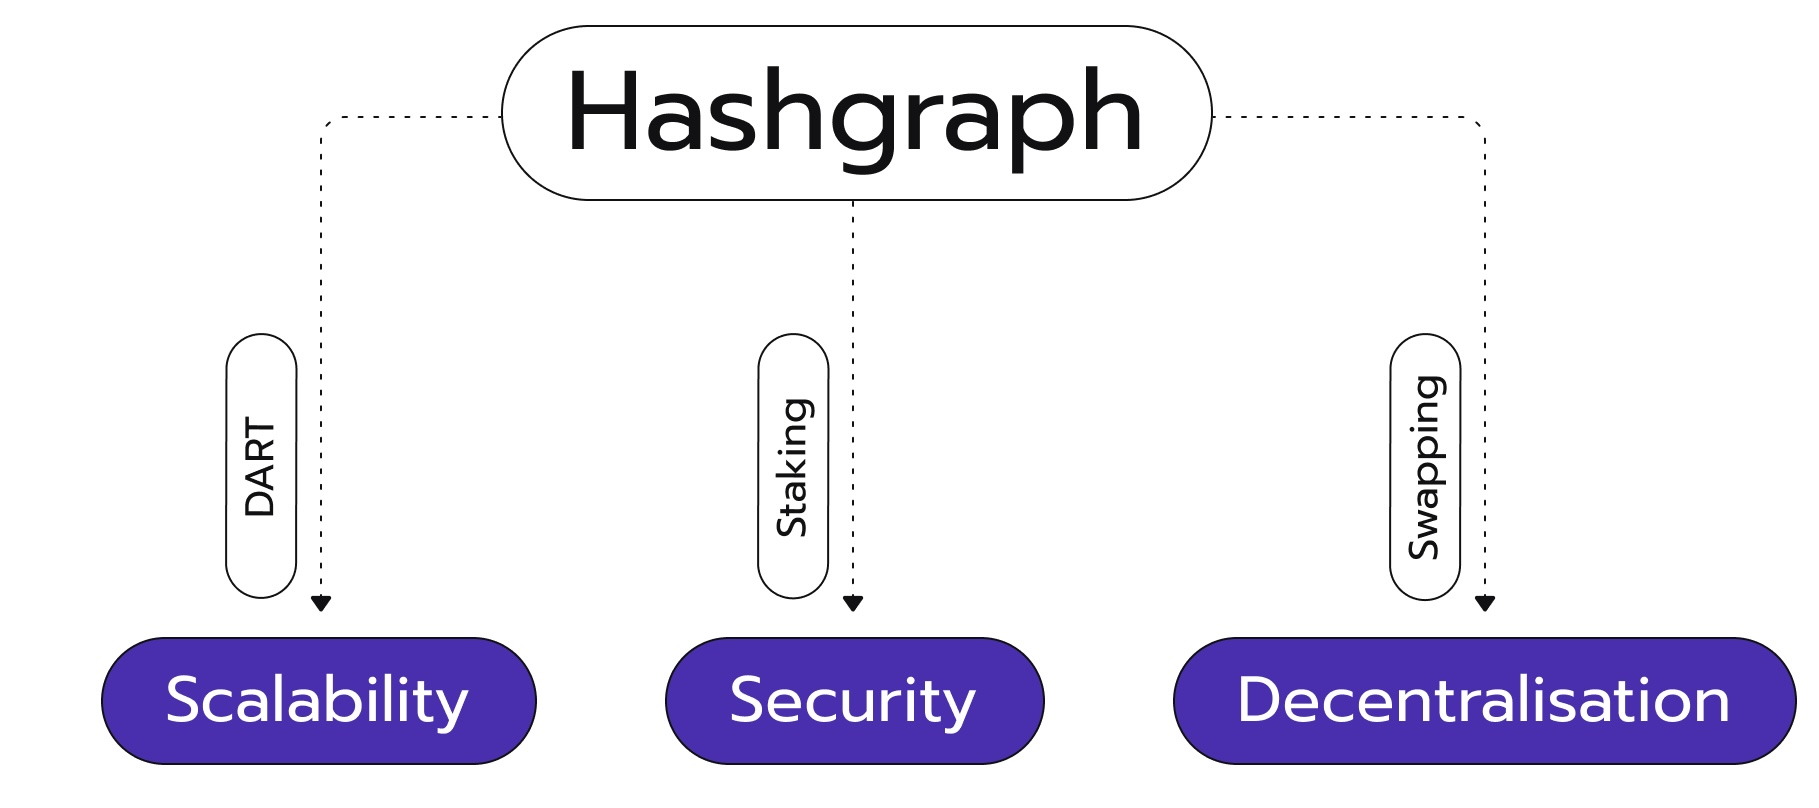
\includegraphics[width=1\textwidth]{figures/paper_structure.jpeg}
        \caption{How Tagion uses its \textit{4 distinguishing features} to solve \textbf{the \gls{trilemma}}.}
        \label{figure:paper_structure}
    \end{figure}

    \subsection{Misconceptions about Distributed Ledgers}
    This paper describes the implementation of a generic \gls{dlt}-system supporting its native \gls{tgn}. It \textit{does not} focus on a specific usage of the \gls{dlt}-system. The definition of \gls{dlt} is evolving and many distinct definitions are present. We adopt the definition of the term "\textit{'ledger' to mean the set of records which are held in common by a substantial proportion of network participants}" \cite{dlt_cam}. A \textit{distributed ledger} is thus a set of records shared between participants in a distributed system, regardless of the purpose and use-cases of the records. Some narrow the definition down to fit their needs, for example to an account-based system storing the history of transactions, but this is neither generic nor constructive \cite{dlt_cam}. Tagion is a \gls{dlt}-system: A distributed, decentralised system agreeing on a common ledger, containing records of arbitrary content. Furthermore, the Tagion system contains records of the current ownership of \gls{tgn}, with a protocol that prevents double-spending of these tokens. 

\pagebreak